%Введение и постановка задачи 
The mitral valve, also known as the bicuspid valve or left atrioventricular
valve, is a valve with two flaps in the heart, that lies between the left atrium
and the left ventricle. The mitral valve and the tricuspid valve are known
collectively as the atrioventricular valves because they lie between the atria
and the ventricles of the heart.\par
\begin{figure}[H]
  \centering
  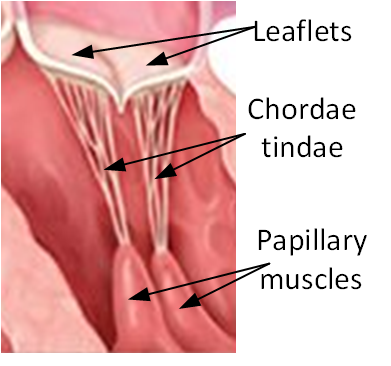
\includegraphics[width=0.4\columnwidth]{./fig/mt.png}
  \caption{Mitral valve structure}
  \label{fig:MT}
\end{figure}
Mitral valve has cyclic working conditions. Blood flows through an open mitral
valve during diastole with contraction of the left atrium, and the mitral valve
closes during systole with contraction of the left ventricle. The valve opens
and closes because of pressure differences, opening when there is greater
pressure in the left atrium than ventricle, and closing when there is greater
pressure in the ventricle than atrium. In abnormal conditions, blood may flow
backwards through the valve (mitral regurgitation) or the mitral valve may be
narrowed (mitral stenosis). Rheumatic heart disease often affects the mitral
valve; the valve may also prolapse with age, and be affected by infective
endocarditis. Mitral valve prolapse (MVP) is a valvular heart disease
characterized by the displacement of an abnormally thickened mitral valve
leaflet into the left atrium during systole. By other words, it is a condition
in which the two flaps of the mitral valve doesn't close smoothly and evenly,
but instead bulge (prolapse) upward into the left atrium.\cite{Hayek2005a}
\begin{figure}[H]\label{fig:compareMT}
  \centering
  \begin{subfigure}[H]{0.42\columnwidth}\label{fig:normalMT}
    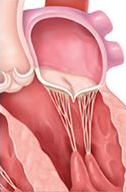
\includegraphics[width=\columnwidth]{./fig/normalMT.png}
    \caption{Normal}
  \end{subfigure}
  \begin{subfigure}[H]{0.4\columnwidth}\label{fig:prolapseMT}
    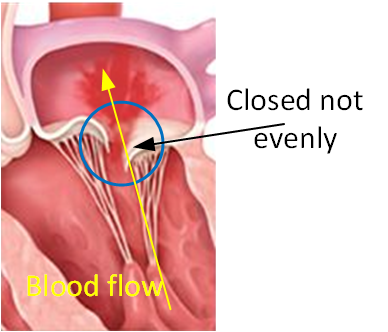
\includegraphics[width=\columnwidth]{./fig/prolapseMT.png}
    \caption{Prolapse}
  \end{subfigure}
  \caption{Comparison of the normal valve and prolapse}
\end{figure}
Providing the surgeon with an anatomically and biomechanically accurate
computional model of a particular patient's mitral heart valve could enable
preoperative surgical planning and potentially improve surgical outcome.\par

